\documentclass[portrait, color=UCLburgundy, margin=1cm]{uclposter}

\linespread{1.0}

\newcommand{\boldf}{\bm{f}}
\newcommand{\boldmu}{\bm{\mu}}
\newcommand{\boldalpha}{\bm{\alpha}}
\newcommand{\boldr}{\bm{r}}
\newcommand{\boldt}{\bm{t}}
\newcommand{\boldg}{\bm{g}}
\newcommand{\boldtheta}{\bm{\theta}}

% Warping operators
\newcommand{\MPWarp}{\tilde{\mathcal{W}}}
\newcommand{\Warp}{\mathcal{W}}

% Others
\newcommand{\etal}{\textit{et al.}~}
\newcommand{\ie}{i.e., }
\newcommand{\eg}{e.g., }

\usepackage{bm}
\usepackage{algorithm}
\usepackage{algorithmic}
\usepackage{caption}
\usepackage{blindtext}
\usepackage{siunitx}

\usepackage{glossaries}

\newacronym{CNN}{CNN}{Convolutional Neural Network}
\newacronym{CT}{CT}{Computed Tomography}
\newacronym{CV}{CV}{Cross Validation}
\newacronym{FOV}{FOV}{Field of View}
\newacronym{ILD}{ILD}{Interstitial Lung Disease}
\newacronym{IPF}{IPF}{Idiopathic Pulmonary Fibrosis}
\newacronym{MB}{MB}{Memory Bank}
\newacronym{MAE}{MAE}{Mean Absolute Error}
\newacronym{NN}{NN}{Neural Network}
\newacronym{OSIC}{OSIC}{Open Source Imaging Consortium}
\newacronym{PReLU}{PReLU}{Parametric Rectified Linear Unit}
\newacronym{RAE}{RAE}{Relative Absolute Error}
\newacronym{STD}{STD}{Standard Deviation}


\usepackage[style=ieee, maxbibnames=1, minbibnames=1, maxcitenames=1, mincitenames=1, backend=biber, defernumbers=false]{biblatex}
\addbibresource{./Biblio.bib}

\AtEveryBibitem{\clearfield{month}}
\AtEveryBibitem{\clearfield{day}}
\AtEveryBibitem{\clearfield{volume}}
\AtEveryBibitem{\clearfield{issue}}
\AtEveryBibitem{\clearfield{pages}}
\AtEveryBibitem{\clearfield{number}}
\AtEveryBibitem{\clearfield{title}}
\AtEveryBibitem{\clearfield{isbn}}
\AtEveryBibitem{\clearfield{keywords}}
\AtEveryBibitem{\clearfield{issn}}
\AtEveryBibitem{\clearfield{journal}}
\AtEveryBibitem{\clearfield{publisher}}

\usepackage{fontspec}
\setmainfont[Ligatures=TeX]{LexendDeca-Regular.ttf}

\begin{document}
    \title{Deep Learning for CT-Based Survival Analysis of Idiopathic Pulmonary Fibrosis Patients}
    
    \author[1, *]{Alexander~C.~Whitehead}
    \author[1, 2]{Ahmed~H.~Shahin}
    \author[1, 2]{An~Zhao}
    \author[1, 2]{Daniel~C.~Alexander}
    \author[3]{\newline Joseph~Jacob}
    \author[1, 4]{David~Barber}
    
    \affil[1]{Department of Computer Science, UCL}
    \affil[2]{CMIC, UCL}
    \affil[3]{Lungs for Living Research Centre, UCL\newline}
    \affil[4]{Centre for Artificial Intelligence, UCL\newline}
    \affil[*]{alexander.whitehead.18@ucl.ac.uk}
    
    \maketitle

    \begin{multicols}{2}
        \section*{Introduction}
            \begin{highlightbox}[UCLlightgreen]
                \begin{itemize}
                    \item \gls{IPF} is characterised by a buildup of scar tissue in and a stiffening of the lungs of the patient.
                    
                    \item \gls{IPF} leads to a reduction in the volume of the lung, a shortness of breath, and eventually death.
                    
                    \item The progression of \gls{IPF} is heterogeneous and prognosis is challenging~\cite{King2011IdiopathicFibrosis}.
                    
                    \item Methods to monitor \gls{IPF} include:

                    \begin{itemize}
                        \item Testing lung function with spirometric measurement of lung volume~\cite{Watters1986AFibrosis}.
                        
                        \item Taking \gls{CT} acquisitions over time~\cite{Lynch2018DiagnosticPaper}.
                    \end{itemize}
                    
                    \item These approaches are limited by several factors, including:

                    \begin{itemize}
                        \item Physical limitations of the patient.
                        
                        \item Technical accuracy (spirometer baseline drift bias).
                        
                        \item Longitudinal data availability.
                    \end{itemize}

                    \item Here, a number of survival analysis methods that predict death time using a neural network are presented.

                    \item Censoring is a significant issue in survival analysis in which the precise death time of a patient is unknown.
                    
                    \item Cox Proportional Hazards Survival Analysis~\cite{Cox1972RegressionLife-Tables} compares the death time of one patient to another ranking according to their expected death times.

                    \begin{itemize}
                        \item A limitation is that the model does not directly output survival times.
                    \end{itemize}

                    \item DeepHit treats survival analysis as a multi-class classification problem with a class for each time-bin that a patient could die in~\cite{Lee2018DeepHit:Risks}.
                    
                    \begin{itemize}
                        \item A disadvantage is that the model is penalised as much for making an error of one month as it is an error of ten years.
                    \end{itemize}

                    \item Here, different training losses are used, including:

                    \begin{itemize}
                        \item Likelihood -  One where censoring time is sampled from a uniform distribution and one where censoring time is sampled in the classical way is used~\cite{Shahin2023DeepAnalysis}.
                        
                        \item Cox based ranking - One with and one without a \gls{MB}.
                        
                        \item DeepHit.
                    \end{itemize}
                \end{itemize}
            \end{highlightbox}

        \section*{Methods}
            \subsection*{\underline{\textbf{Data Acquisition and Preparation}}}
                \begin{itemize}
                    \item 550 \gls{CT} acquisitions from the \gls{OSIC} data set~\cite{OSICOSICRepository}.
                    
                    \item Segmented to remove data outside of the lung.
                    
                    \item Normalised independently.
                    
                    \item Where appropriate, clinical features, such as age and sex were also used.
                    
                    \item Missing clinical features were imputed following~\cite{Shahin2022SurvivalData}.
                    
                    \item Data were split into train and test groups using five fold cross validation.
                \end{itemize}

        \begin{table}[H]
            \centering
            
            \captionsetup{singlelinecheck=false, justification=centering}
            \begin{highlightbox}[UCLlightblue]
                \caption{
                    A comparison of \gls{MAE}, \gls{RAE}, the concordance index, and the Brier score. The average survival time was approximately 32 months. Here, EC Likelihood refers to Event Conditional Likelihood, C Likelihood refers to Classical Likelihood, and CF refers to when the clinical features were included in the model.
                }
            \end{highlightbox}
            
            \resizebox*{1.0\linewidth}{!}
            {
                \begin{tabular}{||c|cc|c|c||}
                    \hline
                                                & \textbf{\gls{MAE}}    & \textbf{\gls{RAE}}    & \textbf{C-Index}  & \textbf{Brier}    \\
                    \hline
                    \textbf{EC Likelihood}      & $22.7\pm1.51$         & $1.72\pm0.89$         & $0.77\pm0.05$     & $0.22\pm0.07$     \\
                    \textbf{EC Likelihood CF}   & $21.5\pm1.32$         & $1.98\pm0.82$         & $0.80\pm0.03$     & $0.18\pm0.05$     \\
                    \textbf{C Likelihood}       & $28.9\pm1.96$         & $2.23\pm0.01$         & $0.76\pm0.05$     & $0.25\pm0.01$     \\
                    \textbf{C Likelihood CF}    & $25.3\pm1.74$         & $2.04\pm0.01$         & $0.75\pm0.04$     & $0.20\pm0.01$     \\
                    \hline
                    \textbf{Cox}                & $187 \pm309 $         & $17.0\pm30.7$         & $0.73\pm0.04$     & $0.61\pm0.28$     \\
                    \textbf{Cox CF}             & $233 \pm287 $         & $26.4\pm21.9$         & $0.72\pm0.03$     & $0.57\pm0.16$     \\
                    \textbf{Cox \gls{MB}}       & $166 \pm267 $         & $17.7\pm28.2$         & $0.74\pm0.03$     & $0.53\pm0.31$     \\
                    \textbf{Cox \gls{MB} CF}    & $179 \pm294 $         & $16.3\pm22.8$         & $0.73\pm0.05$     & $0.56\pm0.24$     \\
                    \hline
                    \textbf{DeepHit}            & $38.4\pm14.8$         & $3.99\pm0.34$         & $0.72\pm0.03$     & $0.40\pm0.01$     \\
                    \textbf{DeepHit CF}         & $31.3\pm9.19$         & $3.50\pm0.42$         & $0.71\pm0.04$     & $0.42\pm0.01$     \\
                    \hline
                \end{tabular}
            }
        \end{table}
    \end{multicols}

    \begin{figure}[H]
        \centering

        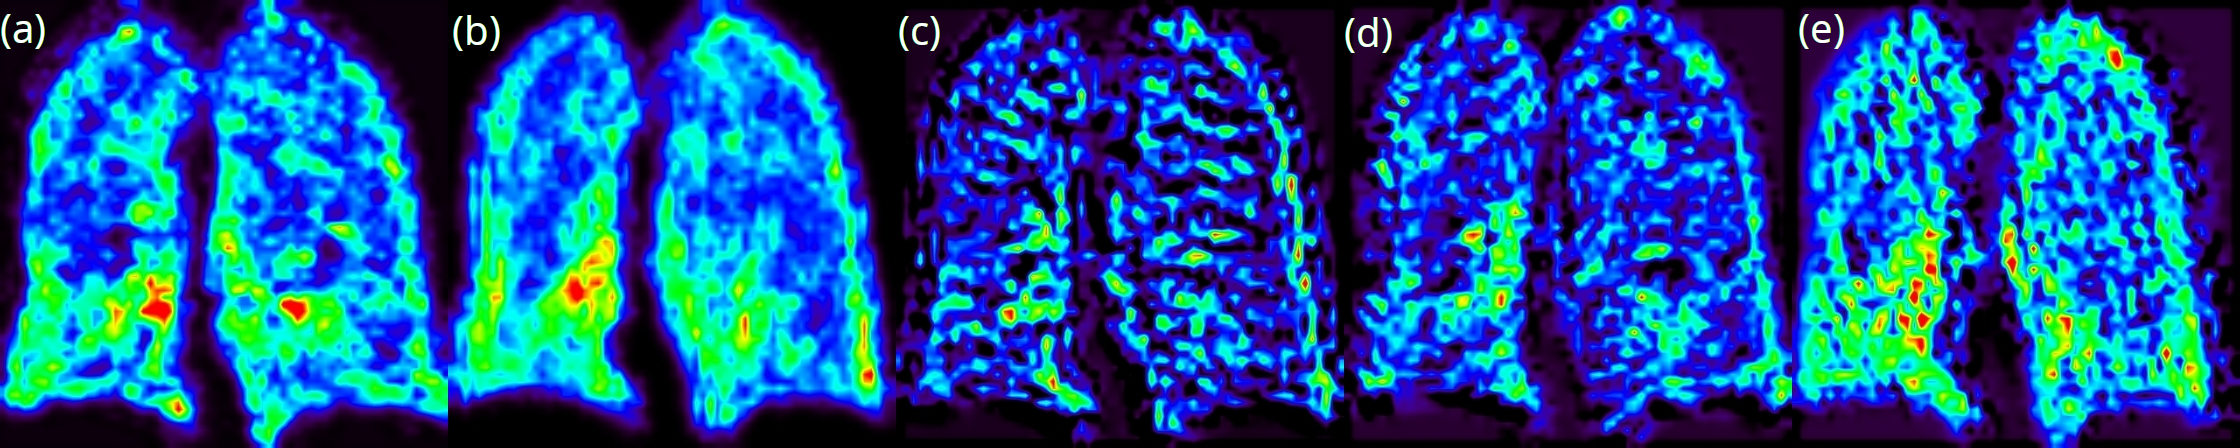
\includegraphics[width=1.0\linewidth]{grad_cam_label.png}
        
        \captionsetup{singlelinecheck=false, justification=centering}
        \begin{highlightbox}[UCLlightblue]
            \caption{
                From left to right a slice through a fibrotic region of a Grad-CAM image, taken from a middle convolution, of a 65 year old patient with a survival time of 30 months. For (a) Event Conditional Likelihood, (b) Classical Likelihood, (c) Cox, (d) Cox \gls{MB}, and (e) DeepHit. All colour maps are consistent for all images.
            }
        \end{highlightbox}
    \end{figure}

    \begin{multicols}{2}
            \subsection*{\underline{\textbf{Models}}}
                \begin{itemize}
                    \item For details of model design see proceeding.
            
                    \item For comparison, five loss functions were trialed:
            
                    \begin{itemize}
                        \item \underline{\textbf{Event Conditional Likelihood}} - Maximise likelihood using a Gaussian to model the time of death, where the censoring time was sampled from a uniform distribution from time zero up to the death time~\cite{Shahin2023DeepAnalysis}.
            
                        \item \underline{\textbf{Classical Likelihood}} - Maximise likelihood using a Gaussian to model the time of death, where the censoring time was sampled from a Gaussian distribution parameterised by the censor time.
            
                        \item \underline{\textbf{Cox}} - Cox Proportional Hazards~\cite{Cox1972RegressionLife-Tables}.
            
                        \item \underline{\textbf{Cox \gls{MB}}} - Cox Proportional Hazards with \gls{MB}~\cite{Shahin2022SurvivalData}.
            
                        \item \underline{\textbf{DeepHit}} - Log-likelihood, with a maximum output value of 105 years and 840 bins~\cite{Lee2018DeepHit:Risks}.
                    \end{itemize}
            
                    \item For both likelihood losses a fixed standard deviation equal to one year was used.
                    
                    \item For both Cox losses the output was converted to survival times using the Breslow estimator~\cite{Breslow1974CovarianceData}.
                \end{itemize}

            \subsection*{\underline{\textbf{Evaluation}}}
                \begin{itemize}
                    \item For evaluation the following was used:

                    \begin{itemize}
                        \item The \gls{MAE} and \gls{RAE} for the uncensored data between the predicted and true value was taken.
                        
                        \item The concordance index.
                        
                        \item The Brier score.
                        
                        \item A visual analysis of Grad-CAM images~\cite{Selvaraju2020Grad-CAM:Localization}.
                    \end{itemize}
                \end{itemize}
                
        \section*{Conclusion}
            \begin{highlightbox}[UCLlightgreen]
                \begin{itemize}
                    \item From evaluation of the results it appears that the likelihood methods provide the best results most often.
                    
                    \item The model used for the DeepHit loss had more parameters (due to the output being larger). Even so, the method does not provide results better than the likelihood methods.
                    
                    \item When clinical features were used it seems to improve results, although not greatly.

                    \item Computation times are as follows:

                    \begin{itemize}
                        \item The likelihood losses and the Cox loss without \gls{MB} are the fastest to compute.
                        
                        \item The DeepHit loss takes slightly longer than previous methods.
                        
                        \item The Cox \gls{MB} loss takes magnitudes longer than all other methods.
                    \end{itemize}
                \end{itemize}
            \end{highlightbox}
        
        \AtNextBibliography{\small}
        \printbibliography
    \end{multicols}
\end{document}
